%!TEX root = ../memoria.tex

\chapter{Pruebas}

Según IEEE (2004), "las pruebas de software "consisten en verificar el comportamiento de un programa dinámico a través de un grupo finito de casos de prueba, debidamente seleccionados del, típicamente, ámbito de ejecuciones infinito, en relación al comportamiento esperado".

Es importante mencionar que bajo una lógica de TDD, las actividades de pruebas son realizadas a lo largo de todo el proyecto e intercaladas con el resto de las actividades de desarrollo, tomando en cuenta la calidad del software a lo largo de toda la vida del proyecto. 


\section{Estructura de las pruebas}

Para la implementación y creación de las pruebas se deben seguir una serie de etapas que garantizan que estas tengan éxito al encontrar los posibles errores en el sistema. A continuación, se detallan las etapas del proceso de prueba del sistema.

\subsection{Planificación}

Esta etapa debe comenzar junto con la planificación del proyecto. Los detalles del plan de pruebas deben ser desarrollados después de la aprobación de la especificación de requerimientos.

En esta etapa se deben definir todos los elementos necesarios para posteriormente llevar acabo las pruebas, esto implica definir los niveles, tipos, metodologías, requerimientos, valores de aprobación y rechazo, recursos materiales y humano, además de responsables del proceso de pruebas.

Las pruebas que serán realizadas deben encontrarse trazadas con los requerimientos previamente aprobados, esto con el fin de asegurar el cumplimiento de todo lo establecido en la toma de requerimientos.

Una vez el documento con el plan de pruebas se encuentre terminado debe ser sometido a revisión y corregido para resolver discrepancias con el plan de proyecto, considerando los plazos y recomendaciones.

\subsection{Especificación}

Basado en el plan de pruebas desarrollado en la etapa anterior se debe describir con mayor rigor cada uno de los test que se realizaran identificando el propósito, los métodos y contenidos de las entradas y salidas.

Es importante detallar con exactitud los métodos y contenido de \textit{input} y \textit{output} del sistema, describiendo los tipos y volúmenes de datos; rangos de capacidad y tiempos de respuesta; métodos que serán utilizados para ingresar y recibir la información; y la traza con los requerimientos para aprobar o rechazar una funcionalidad específica del sistema.

Junto a lo anterior, es necesario definir los métodos y herramientas que deben utilizarse y describir el proceso de análisis de los resultados.
Considerando que en este punto el sistema se encuentra en una etapa temprana de desarrollo, los niveles de prueba deben ser descritos en el siguiente orden: sistema, aceptación, integración y unitarias.

Al igual que en la etapa anterior, el documento debe ser revisado, corregido de ser necesario y aprobado. 
Las pruebas de sistema realizan una comparación entre los objetivos originales del sistema, aquellos planteados en la toma de requisitos, y los procesos, actividades y rutinas del sistema desarrollado.

\subsection{Ejecución}

Basado en la especificación de las pruebas descritas en la etapa anterior, se debe realizar la ejecución de cada uno de los test, registrando los resultados y estableciendo, para cada prueba, el éxito o fracaso en base a los criterios ya definidos. 

En caso de que el sistema no apruebe alguna de las pruebas, el equipo de desarrollo debe encargarse de realizar las correcciones necesarias y posteriormente se debe comprobar la correctitud del sistema completo. 
Una vez el sistema apruebe todas las pruebas, se debe seguir con la siguiente actividad definida en el plan de pruebas. 

Las pruebas se deben realizar en el siguiente orden.

\begin{itemize}
	\item
		\textbf{Pruebas unitarias:} En paralelo a la etapa de codificación.
	\item
		\textbf{Pruebas de integración:} En paralelo a la etapa de integración.
	\item 
		\textbf{Pruebas del sistema:} Previo a la entrega del sistema.
	\item
		\textbf{Pruebas de aceptación:} Antes de la etapa de aceptación y entrega.
\end{itemize}

Únicamente las pruebas unitarias son responsabilidad del equipo de desarrollo, el resto debe ser realizadas por un equipo distinto, responsable de estas.

\subsection{Análisis de resultados}

Basado en los resultados obtenidos, se debe realizar un análisis que permita identificar los defectos y sus posibles causas, lo anterior con el objetivo de establecer acciones correctivas y evitar propagación y repetición de errores.

Es importante recalcar que no se deben buscar responsabilidades individuales, únicamente asociar el fallo con un proceso en el desarrollo.

\subsection{Completación}

Para dar conclusión al proceso de prueba, la unidad responsable debe preparar los elementos necesarios para su posterior uso y realizar la documentación del proceso realizado.

\section{Pruebas sobre el sistema \textit{Gerprin}}

A continuación, se describen los tipos de pruebas que deben ser realizadas sobre el sistema \textit{Gerprin}. 

\subsection{Pruebas unitarias}

Las pruebas unitarias tienen como objetivo asegurar que cada una de las funciones codificadas para el sistema realicen de forma correcta el proceso para el cual fueron creadas. Este tipo de pruebas se realiza bajo la lógica de “caja blanca”, debido a la necesidad de probar las excepciones, casos de error, validaciones de los datos de entrada y mensajes posibles de respuesta.

Si bien las pruebas unitarias son responsabilidad del equipo de desarrollo, la instancia final de estas debe ser realizadas por personas distintas a quienes se encargaron de codificar la función que debe ser probada.

Basado en la metodología TDD, descrita con anterioridad, el tipo de pruebas descritas en esta sección deben ser realizadas en paralelo al proceso de codificación y marcan el fin de cada una de las iteraciones de esta etapa al ser aprobadas.

Se debe particionar cada uno de los procesos en unidades funcionales y definir las pruebas para los casos de éxito y posibles caminos alternativos. Las pruebas unitarias concluyen una vez se probaron las funciones codificadas hasta el momento, es decir, las completadas en la misma iteración e iteraciones anteriores del desarrollo. 


\subsubsection{Herramientas}

La gran mayoría de \textit{framwork} permiten la automatización de pruebas unitarias para agilizar el proceso y reducir errores humanos. Adicionalmente, software como \textit{Postman} o \textit{SoapUI} permiten hacer consultas mediante \textit{SOAP} o \textit{REST} de forma automática, convirtiéndose en herramientas muy útiles en esta etapa de pruebas.

\subsubsection{Documentación}

Las pruebas unitarias, al igual que el resto, deben ser correctamente documentadas, tanto su planificación como los resultados obtenidos. Adicionalmente, para este tipo de pruebas se debe documentar la traza con los requisitos funcionales, especificando explícitamente que a cuál requisito corresponde la función que se encuentra probando.

Las plantillas para la documentación de las pruebas unitarias se encuentran en anexos.

\subsubsection{Ejemplo de prueba}

A continuación, se presenta un ejemplo de prueba unitaria utilizando \textit{Postman} para la comprobación de las respuestas de la \textit{API} y el correcto funcionamiento de esta. Las respuestas aquí esperadas deben ser redefinidas y aceptadas por el equipo de desarrollo como las esperadas por el sistema, debido a que estas se encuentran basadas en el primer desarrollo de Gerprin y no en las nuevas funcionalidades que serán creadas.

Para agilizar el proceso se deben automatizar las pruebas unitarias que se ejecutaran, esto debido a la gran cantidad de funcionalidades que componen un sistema con las características de \textit{Gerprin}. \textit{Postman} permite validar la información recibida de una solicitud tipo \textit{REST} mediante \textit{Javascript}. Se debe registrar en la documentación pertinente el código utilizado para validar las solicitudes en la sección correspondiente.

La siguiente prueba se realizará sobre la función de \textit{update\_user} que permite modificar los datos del usuario que corresponden a nombre, apellido y rut. Para realizar la prueba se deben encadenar dos solicitudes, la primera de tipo \textit{POST} a \textit{update\_user}, que permite modificar los datos del usuario y la segunda de tipo \textit{GET} a \textit{get\_user}, que retorna la información de un usuario entregando el \textit{ID} de este, posteriormente se realizara nuevamente ambas solicitudes con nuevos datos para comprobar que efectivamente se realizó la modificación de la información y no fue una coincidencia que la información inicial del usuario coincidiera con la primera prueba.

El proceso de creación del tests automático debe ser realizado antes del proceso de pruebas, pero se añadirá en el siguiente cuadro con el propósito de ejemplificar de mejor forma las pruebas unitarias.

\begin{table}[H]
    \caption[Ejemplo pruebas unitarias] {Ejemplo pruebas unitarias}
    \label{tbl:ejemplo pruebas unitarias}
    \begin{tabular}{|p{1\textwidth}|}
        \hline
        \textbf{Prueba Unitaria: Actualizar Usuario Caso exitoso. \hfill ID: 10} \\
    	\hline
    	\hline
    	\textbf{Caso de prueba:} Update User \\
    	\hline
    	\textbf{Requisito Funcional asociado:} Fiabilidad \\
    	\hline
    	\textbf{Propósito:} Se probará que las solicitudes de \textit{update\_user} acepten correctamente el formato de los datos de entrada y retornen el resultado esperado. \\
    	\hline
    	\textbf{Prerrequisitos: }
		se debe encontrar creadas las variables globales que utilizara Postman . Las variables a crear son:
		\begin{itemize}
			\item \textit{url\_base}: Corresponde a la ruta base donde se encuentra montado el sistema, por ejemplo, “localhost:8080/”
			\item \textit{apikey}: clave que permite el uso de la \textit{API}. 
			\item \textit{id\_user}: Número identificatorio del usuario que será modificado.
			\item \textit{name\_user}: Nombre del usuario que será modificado. 
			\item \textit{lastname\_user}: Apellido del usuario que será modificado.
			\item \textit{rut\_user}: Rut del usuario que será modificado.
			\item \textit{name\_user\_2}: Nombre del usuario que será modificado, distinto a la variable \textit{name\_user}.
			\item \textit{Lastname\_user\_2}: Apellido del usuario que será modificado, distinto a la variable \textit{lastname\_user}.
			\item \textit{rut\_use\_2}: Rut del usuario que será modificado, distinto a la variable \textit{rut\_user}.
			\item \textit{debe} tener instalado \textit{Postman v7.2.2} y el sistema en un entorno local, de \textit{playground} o \textit{staged}
		\end{itemize} \\ \hline
		\textbf{Datos de entrada: }
		se debe encontrar creadas las variables globales que utilizara Postman . Las variables a crear son:
		\begin{itemize}
			\item Primera solicitud
			\begin{itemize}
				\item url: \{\{url\_base\}\}update\_user
				\item Método: POST
				\item head
				\begin{itemize}
					\item X-API-Key: \{\{apikey\}\}
					\item Content-Type: application/json
				\end{itemize}
				\item body
				\begin{itemize}
					\item id: \{\{id\}\}
					\item name\_user: \{\{name\_user\}\}
					\item lastname\_user: \{\{lastname\_user\}\}
					\item rut\_user: \{\{rut\_user\}\}
				\end{itemize}
			\end{itemize}
			\item Segunda solicitud
			\begin{itemize}
				\item url: \{\{url\_base\}\}get\_user
				\item Método: GET
				\item head
				\begin{itemize}
					\item X-API-Key: \{\{apikey\}\}
					\item Content-Type: application/json
				\end{itemize}
				\item body
				\begin{itemize}
					\item id: \{\{id\}\}
				\end{itemize}
			\end{itemize}
		\end{itemize} \\ \hline
    \end{tabular}
\end{table}

\begin{table}[H]
    \begin{tabular}{|p{1\textwidth}|}
    	\hline
		\begin{itemize}
			\item Tercera solicitud
			\begin{itemize}
				\item url: \{\{url\_base\}\}update\_user
				\item Método: POST
				\item head
				\begin{itemize}
					\item X-API-Key: \{\{apikey\}\}
					\item Content-Type: application/json
				\end{itemize}
				\item body
				\begin{itemize}
					\item id: \{\{id\}\}
					\item name\_user: \{\{name\_user\_2\}\}
					\item lastname\_user: \{\{lastname\_user\_2\}\}
					\item rut\_user: \{\{rut\_user\_2\}\}
				\end{itemize}
			\end{itemize}
			\item Cuarta solicitud
			\begin{itemize}
				\item url: \{\{url\_base\}\}get\_user
				\item Método: GET
				\item head
				\begin{itemize}
					\item X-API-Key: \{\{apikey\}\}
					\item Content-Type: application/json
				\end{itemize}
				\item body
				\begin{itemize}
					\item id: \{\{id\}\}
				\end{itemize}
			\end{itemize}
		\end{itemize} \\ \hline
		\textbf{Pasos:}
		\begin{itemize}
			\item Crear o importar las variables globales a utilizar
			\item En caso de no encontrarse creada la colección de solicitudes debe ser creada.
			\item Se crea la colección en la pestaña \textit{“Collections”} con nombre \textit{“Actualizar Usuario Caso exitoso”}
			\item Se crean las request de la colección
			\begin{itemize}
				\item Creamos la solicitud en el menu desplegable de la colección (click con boton derecho sobre la colección, luego en \textit{“add request”}). Se añade nombre  y descripción.
				\item Abrir la solicitud e ingresar los parámetros de url, método, \textit{head} y \textit{body}
				\item En la pestaña test se añade el código que comprueba que los resultados son correctos.
			\end{itemize}
			\item Correr colección de solicitudes
		\end{itemize} \\ \hline
		\textbf{Resultados esperados:} Se espera que la totalidad de los resultados sean \textit{“OK”}\\
		Solicitud 1:
		\begin{verbatim}
			tests["Status code is 200"] = responseCode.code === 200;
			var data = JSON.parse(responseBody);
			tests["Message: " + data.message] = data.message === "User successfully update";
			tests["Id user update"] = responseBody.has("id") === pm.environment.get("id_user”);

		\end{verbatim}

		Solicitud 2:
		\begin{verbatim}
			tests["Status code is 200"] = responseCode.code === 200;
			var data = JSON.parse(responseBody);
			tests["Id User"] = responseBody.has("id") === pm.environment.get("id_user”);
			tests["Name User"] = responseBody.has("name") === pm.environment.get("name_user”);
			tests["Lastname User"] = responseBody.has("lastname") === 
				pm.environment.get("lastname_user”);
			tests["Rut User"] = responseBody.has("rut") === pm.environment.get("rut_user”);

		\end{verbatim}

		Solicitud 3:
		\begin{verbatim}
			tests["Status code is 200"] = responseCode.code === 200;
			var data = JSON.parse(responseBody);
			tests["Message: " + data.message] = data.message === "User successfully update";
			tests["Id user update"] = responseBody.has("id") === pm.environment.get("id_user”);
		\end{verbatim}
		\\ \hline
    \end{tabular}
\end{table}

\begin{table}[H]
    \begin{tabular}{|p{1\textwidth}|}
    	\hline
		Solicitud 4:
		\begin{verbatim}
			tests["Status code is 200"] = responseCode.code === 200;
			var data = JSON.parse(responseBody);
			tests["Id User"] = responseBody.has("id") === pm.environment.get("id_user);
			tests["Name User"] = responseBody.has("name") === pm.environment.get("name_user_2”);
			tests["Lastname User"] = responseBody.has("lastname") === 
			pm.environment.get("lastname_user_2”);
			tests["Rut User"] = responseBody.has("rut") === pm.environment.get("rut_user”);
 
		\end{verbatim}  
		
		\\ \hline
		\textbf{Resultado Obtenido:}\\
		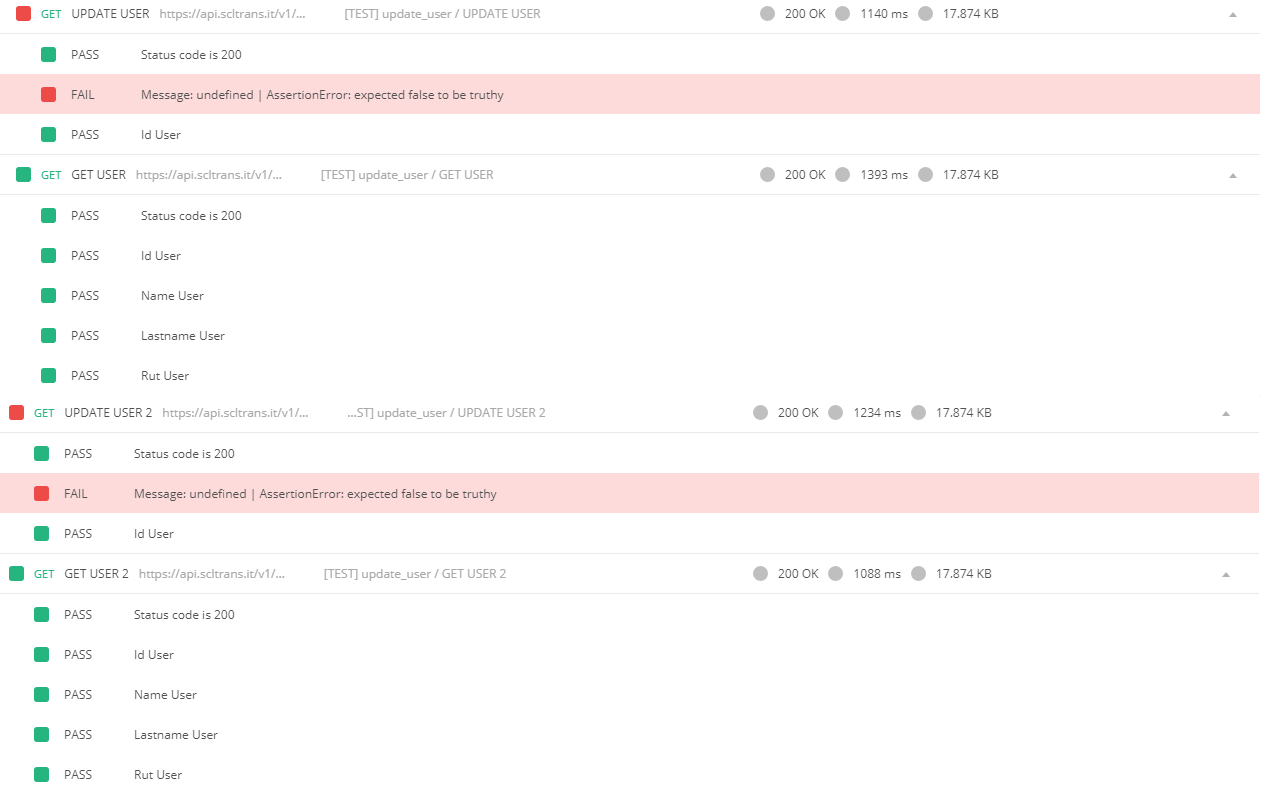
\includegraphics[width=15cm]{figures/Respuestapruebasunitarias.png}
		\\ \hline
    \end{tabular}
\end{table}

\subsection{Pruebas de integración}

Las pruebas de integración aseguran el correcto funcionamiento entre dos o más unidades del sistema, para \textit{Gerprin} es clave el acoplamiento entre los distintos módulos que lo componen para asegurar estándares de calidad mínimos asociados a mantenibilidad y fiabilidad de datos.

La integración entre las unidades es dependiente del ambiente en el cual se encuentre el sistema, por lo que se debe montar un entorno de preproducción, también conocido como ambiente de \textit{staging} o de \textit{QA}. Este ambiente debe tener las mismas características que producción para evitar futuros problemas de compatibilidad.

Este tipo de pruebas son realizadas por el área de \textit{QA} y se encarga tanto de realizar las pruebas como de documentarlas. Por su parte, el equipo de desarrollo se debe encargar de entregar las instrucciones necesarias para levantar el servicio en \textit{staging} y dar el soporte de ser necesario.

Las pruebas de integración seguirán la lógica \textit{down-top}, es decir, se llamarán los módulos superiores (\textit{API}) desde los módulos inferiores (aplicación móvil y modulo abordo). Se debe cuidar que la base de datos de prueba sea consistente y considerar que las soluciones deben ser de carácter global, debido a que afectan a la comunicación entre módulos, por ejemplo, si se decide cambiar la comunicación de \textit{REST} a \textit{SOAP}, se debe considerar hacerlo en todas las llamadas de dicho modulo para mantener la coherencia del sistema.


\subsubsection{Herramientas}

Para la creación de un entorno de pruebas es altamente recomendable emplear \textit{Vagrant} o \textit{Docker} para emular un servidor de producción, esto debido a que permiten crear maquinas virtuales o contenedores que de forma rápida pueden copiar las características de los servidores de producción.

\subsubsection{Documentación}

Respecto a la documentación de las pruebas de integración es necesario identificar las unidades que se pondrán a prueba.

Las plantillas para la documentación de las pruebas de integración se encuentran en anexos.

\subsubsection{Ejemplo de prueba}

El siguiente ejemplo prueba la misma funcionalidad antes propuesta, sin embargo, la prueba debe ser realizada desde la aplicación con interfaz gráfica. La importancia de la prueba de integración radica en la comunicación entre los distintos módulos.

\begin{table}[H]
    \caption[Ejemplo pruebas de integración.] {Ejemplo pruebas de integración.}
    \label{tbl:Ejemplo pruebas de integración}
    \begin{tabular}{|p{1\textwidth}|}
        \hline
        \textbf{Prueba de Integracion: Actualizar Usuario caso exitoso. \hfill ID: 10} \\
    	\hline
    	\hline
    	\textbf{Caso de prueba:} Update User\\ \hline
    	\textbf{Unidades relacionadas:} Modulo API, Aplicación móvil y lector biométrico\\ \hline
    	\textbf{Propósito:} Se probará que los usuarios puedan modificar su información.\\ \hline
    	\textbf{Prerrequisitos:} El sistema debe encontrarse en ambiente de \textit{staged}. La base de datos de prueba debe tener un usuario cargado con nombre, apellido y Rut distintos a los indicados en los datos de entrada\\ \hline
		\textbf{Datos de entrada:} Se deben ingresar de forma manual los siguientes datos:
		\begin{itemize}
			\item Nombre “Elizabeth”
			\item Apellido “Sánchez”
			\item Rut “123456780”
		\end{itemize} \\ \hline
		\textbf{Pasos:} 
		\begin{itemize}
			\item Realizar login en la aplicación
			\item Ir a mi perfil (esquina superior izquierda) 
			\item Ir a editar datos
			\item Ingresar datos
			\item Click en guardar
			\item Comprobar que los datos fueron modificados en base de datos manejada por la API
			\item Comprobar que los datos se muestran modificados en la aplicación (perfil de usuario, datos que se muestran por defecto en la pantalla de editar usuario y detalle de usuario en pantalla de administrador)
			\item Comprobar que los datos se muestran modificados en la pantalla led del lector biométrico
		\end{itemize}\\ \hline
		\textbf{Resultados esperados:} El sistema debe redirigir a la página del perfil de usuario mostrando los nuevos datos e indicar que se guardaron exitosamente los datos. \\ \hline
		\textbf{Resultado obtenido:} El sistema redirige a la página con los nuevos datos, pero no muestra mensaje indicando que el cambio fue exitoso.\\ \hline
    \end{tabular}
\end{table}

La prueba anterior comprueba la correcta comunicación entre la aplicación móvil y la \textit{API}, La \textit{API} y base de datos, \textit{API} y modulo a bordo. 

\subsection{Pruebas de sistema}

Las pruebas de sistema son la última instancia para identificar errores antes de entregar el software al cliente, este proceso se realiza sobre el producto completo. Estas pruebas engloban un conjunto de tests que aseguran la correcta implementación de las reglas de negocio, para esto comprueba la navegación del sistema, el ingreso de datos, procesamiento y recuperación. Para el caso de \textit{Gerprint}, se implementarán pruebas performance y de humo.

Las pruebas de performance intentan emular el tráfico normal de uso que se encontrara la aplicación, se debe realizar para cada una de las funciones del sistema. Mientras que las pruebas de humo corresponden a pruebas no exhaustivas del sistema completo, además, se debe considerar dentro de las pruebas de humo, que la aplicación cumpla con las condiciones de usabilidad para los tamaños de los distintos dispositivos especificados 
 

\subsubsection{Documentación}

Las pruebas de performance deben documentar la cantidad de solicitudes por minuto realizadas a la aplicación, tiempo de respuesta y uso de ram y procesador del servidor. 

Las plantillas para la documentación de las pruebas de humo se encuentran en anexos

\subsubsection{Ejemplo de prueba}

Las pruebas de sistema se hacen contra el documento de requisitos. Cada una de las pruebas realizadas debe hacer referencia a uno de los requerimientos identificados en la etapa de análisis.

\begin{table}[H]
    \caption[Ejemplo pruebas de hummo] {Ejemplo pruebas de hummo}
    \label{tbl:ejemplo pruebas de humo}
    \begin{tabular}{|p{1\textwidth}|}
        \hline
        \textbf{Prueba de Humo: Actualizar Usuario caso exitoso. \hfill ID: 10} \\
    	\hline
    	\hline
    	\textbf{Caso de prueba:} Update User\\ \hline
    	\textbf{Requisito:} Update User (ID: 10)\\ \hline
    	\textbf{Prerrequisitos:} El sistema debe encontrarse en ambiente de stage.\\ \hline
		\textbf{Datos de entrada:} Se deben ingresar de forma manual los siguientes datos:
		\begin{itemize}
			\item Nombre “Elizabeth”
			\item Apellido “Sánchez”
			\item Rut “123456780”
		\end{itemize} \\ \hline
		\textbf{Pasos:} 
		\begin{itemize}
			\item Realizar login en la aplicación
			\item Ir a mi perfil (esquina superior izquierda) 
			\item Ir a editar datos
			\item Ingresar datos
			\item Click en guardar
			\item Comprobar que los datos fueron modificados en base de datos manejada por la API
			\item Comprobar que se ajuste a pantallas de 3,5 pulgadas con resolución de 360 x 640 o superior.
			\item Comprobar que los textos tengan un contraste adecuado respecto al fonda para su fácil lectura. 
			\item Comprobar que los iconos tengan relación con la acción a realizar
		\end{itemize}\\ \hline
		\textbf{Resultados esperados:} El sistema debe redirigir a la página del perfil de usuario mostrando los nuevos datos e indicar que se guardaron exitosamente los datos. \\ \hline
		\textbf{Resultado obtenido:} El cliente reporta que el sistema redirige a la página con los nuevos datos, pero no muestra mensaje indicando que el cambie fue exitoso.\\ \hline
    \end{tabular}
\end{table}

\begin{table}[H]
    \caption[Ejemplo pruebas de performance] {Ejemplo pruebas de performance}
    \label{tbl:ejemplo pruebas de performance}
    \begin{tabular}{|p{1\textwidth}|}
        \hline
        \textbf{Prueba performance: Actualizar Usuario caso exitoso.  \hfill ID: } \\
    	\hline
    	\hline
    	\textbf{Caso de prueba:} Update User\\ \hline
    	\textbf{Cantidad de solicitudes por minuto:} 100 solicitudes por segundo \\ \hline
    	\textbf{Propósito:} \\ \hline
    	\textbf{Prerrequisitos: }
		se debe encontrar creadas las variables globales que utilizara Postman . Las variables a crear son:
		\begin{itemize}
			\item \textit{url\_base}: Corresponde a la ruta base donde se encuentra montado el sistema, por ejemplo, “localhost:8080/”
			\item \textit{apikey}: clave que permite el uso de la \textit{API}. 
			\item \textit{id\_user}: Número identificatorio del usuario que será modificado.
			\item \textit{name\_user}: Nombre del usuario que será modificado. 
			\item \textit{lastname\_user}: Apellido del usuario que será modificado.
			\item \textit{rut\_user}: Rut del usuario que será modificado.
			\item \textit{name\_user\_2}: Nombre del usuario que será modificado, distinto a la variable \textit{name\_user}.
			\item \textit{Lastname\_user\_2}: Apellido del usuario que será modificado, distinto a la variable \textit{lastname\_user}.
			\item \textit{rut\_use\_2}: Rut del usuario que será modificado, distinto a la variable \textit{rut\_user}.
			\item \textit{debe} tener instalado \textit{Postman v7.2.2} y el sistema en un entorno local, de \textit{playground} o \textit{staged}
		\end{itemize} \\ \hline
		\textbf{Datos de entrada: }
		se debe encontrar creadas las variables globales que utilizara Postman . Las variables a crear son:
		\begin{itemize}
			\item Primera solicitud
			\begin{itemize}
				\item url: \{\{url\_base\}\}update\_user
				\item Método: POST
				\item head
				\begin{itemize}
					\item X-API-Key: \{\{apikey\}\}
					\item Content-Type: application/json
				\end{itemize}
				\item body
				\begin{itemize}
					\item id: \{\{id\}\}
					\item name\_user: \{\{name\_user\}\}
					\item lastname\_user: \{\{lastname\_user\}\}
					\item rut\_user: \{\{rut\_user\}\}
				\end{itemize}
			\end{itemize}
		\end{itemize}\\ \hline

		\textbf{Tiempo Promedio:} 3,2 segundos\\ \hline
    \end{tabular}
\end{table}

\subsection{Pruebas de aceptación}

Las pruebas de aceptación son realizadas por el cliente y tiene como objetivo validar que se cumplan los requisitos levantados. Estas pruebas se realizan bajo la lógica de “caja negra”, debido a que no es relevante el funcionamiento interno de la aplicación para los usuarios finales. 
El cliente debe poseer el manual de usuario y documento de requisitos para completar las pruebas de aceptación. 



\subsubsection{Documentación}

A diferencia de las pruebas anteriores para el presente tipo de pruebas, se debe llenar los cuadros de información únicamente si el cliente reporta un error en el funcionamiento del sistema.

\subsubsection{Ejemplo de prueba}

\begin{table}[H]
    \caption[Ejemplo pruebas de aceptación] {Ejemplo pruebas de aceptación}
    \label{tbl:ejemplo pruebas de aceptación}
    \begin{tabular}{|p{1\textwidth}|}
        \hline
        \textbf{Prueba de Aceptación: Actualizar Usuario caso exitoso. \hfill ID: 10} \\
    	\hline
    	\hline
    	\textbf{Caso de prueba:} Update User\\ \hline
    	\textbf{Reporte del cliente:} Se reporto el error mediante plataforma de soporte ticket asociado: 0032
			Al editar el usuario, el sistema no me muestra mensaje indicando que fue modificado exitosamente o que ocurrió un error, según se indica en el documento de requerimientos. \\ \hline
    	\textbf{Prerrequisitos:} El sistema debe encontrarse en ambiente de staged. La base de datos de prueba debe tener un usuario cargado con nombre, apellido y Rut distintos a los indicados en los datos de entrada.\\ \hline
		\textbf{Datos de entrada:} Se deben ingresar de forma manual los siguientes datos:
		\begin{itemize}
			\item Nombre “Elizabeth”
			\item Apellido “Sánchez”
			\item Rut “123456780”
		\end{itemize} \\ \hline
		\textbf{Pasos:} 
		\begin{itemize}
			\item Realizar login en la aplicación
			\item Ir a mi perfil (esquina superior izquierda) 
			\item Ir a editar datos
			\item Ingresar datos
			\item Click en guardar
			\item Comprobar que se muestre mensaje indicando estado del cambio realizado, con uno de los siguientes dos mensajes: “Usuario modificado con éxito” o “Error al modificar usuario”  

		\end{itemize}\\ \hline
		\textbf{Resultados esperados:} El sistema debe redirigir a la página del perfil de usuario mostrando los nuevos datos e indicar que se guardaron exitosamente los datos.  \\ \hline
		\textbf{Resultado obtenido:} El cliente reporta que el sistema redirige a la página con los nuevos datos, pero no muestra mensaje indicando que el cambie fue exitoso.\\ \hline
    \end{tabular}
\end{table}